%
% Body text font is Palatino!
%

\documentclass[a5paper,pagesize,10pt,bibliography=totoc,numbers=enddot,
headings=normal,DIV=9,twoside=false,tablecaptionabove]{scrbook}

% twoside, openright
\KOMAoptions{DIV=last}

\usepackage{trajan}
\usepackage{calc} 
\usepackage[french]{babel}
%\usepackage[utf8]{inputenc}
\usepackage[T1]{fontenc}
\usepackage[protrusion=true]{microtype}
\usepackage[babel]{csquotes}
% Désactive l'étiquette de la figure dans les légendes
\usepackage[labelformat=empty,skip=10pt,tableposition=above]{caption}
\usepackage[hidelinks]{hyperref}
\usepackage{booktabs}
\usepackage{tabularx}
\usepackage{graphicx}
\usepackage{zref-savepos}
\usepackage{enumitem}
\setlist[itemize]{topsep=2pt}

\usepackage[table]{xcolor}
\newcommand\colortablerows{%
	\overlock
	\rowcolors{2}{gray!15}{white}
}%
\usepackage{xspace}

% Indentation des paragraphes
\setlength{\parindent}{10pt}
% Sauts de ligne entre les paragraphes
\setlength{\parskip}{1.4ex plus 0.35ex minus 0.3ex}
%\setlength{\parskip}{1.4ex plus 0.35ex minus 0.3ex}

% Pas de numérotation au-delà des chapitres
\setcounter{secnumdepth}{\chapternumdepth}

% Police de caractère générale
\usepackage[sc]{mathpazo}
\linespread{1.05} 
% Police de caractères des titres
\usepackage{LobsterTwo}
\usepackage{overlock}
\addtokomafont{chapter}{\LobsterTwo}
\addtokomafont{disposition}{\overlock}
\addtokomafont{caption}{\overlock}
\setmainfont
     [ BoldFont       = texgyrepagella-bold.otf ,
       ItalicFont     = texgyrepagella-italic.otf ,
       BoldItalicFont = texgyrepagella-bolditalic.otf ]
     {texgyrepagella-regular.otf}

\title{A book title}
\author{Author Name}
\date{2020}

\begin{document}


%=========================================
\makeatletter
\begin{titlepage}
		\centering{
			{\fontsize{40}{48}\selectfont 
			\@title}
		}\\
			
		\vspace{10mm}
		\centering{\Large{\@author}}\\
		\vspace{\fill}
		\centering \large{\@date}
\end{titlepage}
\makeatother

%=========================================
\newpage{}
\thispagestyle {empty}

\vspace*{2cm}

\begin{center}
	\Large{\parbox{10cm}{
		\begin{raggedright}
		{\Large 
			\textit{Do what you think is interesting, 
			do something that you think is fun and worthwhile, 
			because otherwise you won’t do it well anyway.}
		}
	
		\vspace{.5cm}\hfill{---Brian W. Kernighan}
		\end{raggedright}
	}
}
\end{center}

\newcommand\keywords[3]{%
	\section*{Mots-clés :}

	\textbf{Cadre} : #1

	\textbf{Genre} : #2

	\textbf{Thème} : #3
}%

\newcommand\medfan[1]{%
	\emph{medfan}
}%

\newcommand{\filltopageendgraphics}[2][]{%
  \par
  \zsaveposy{top-\thepage}% Mark (baseline of) top of image
  \vfill
  \zsaveposy{bottom-\thepage}% Mark (baseline of) bottom of image
  \def\thisheight{\dimexpr\zposy{top-\thepage}sp-\zposy{bottom-\thepage}sp\relax}
  %\smash{
  \begin{figure}[h]
	\centering
	\includegraphics[height=\ifdim\thisheight<0.3\textheight \thisheight \else 0.3\textheight \fi,#1]{#2}
  \end{figure}
  %}%
  \par
}%

\newcommand\illustration[1]{%
%	\begin{figure}[h]
%		\centering
		\filltopageendgraphics{images/#1}
%	\end{figure}
}%

\newpage


%=========================================
\chapter*{Préambule}

Cet ouvrage est un ensemble de 31 scénarios hétéroclites conçus pour être joués dans des jeux de rôle sur table.
La plupart de ces histoires sont volontairement ouvertes, laissant aux joueurs et joueuses le soin de combler les vides et de préciser les flous par leur imagination.
Grâce à cette liberté d'interprétation, les scénarios ne sont attachés ni à des systèmes spécifiques, ni à des univers particuliers.
Les différentes aventures font donc la part belle à l'improvisation.

Chaque scénario est décrit par trois mots-clés :
\begin{itemize}
	\item le cadre dans lequel il a été imaginé,
	\item le genre d'histoire racontée,
	\item le thème de l'aventure.
\end{itemize}

Un index en fin d'ouvrage permet de retrouver la liste des scénarios relevant des différents mots-clés.
Ceux-ci sont toutefois à prendre comme des indications et non des obligations.
La plupart des aventures peuvent aisément être transposées d'un cadre à un autre voire d'un genre à un autre.

Les scénarios sont divisés en trois sous-parties: l'accroche, les péripéties et la résolution.
L'accroche, plus ou moins longue, pose la situation initiale dans laquelle se trouvent les personnages.
Les péripéties forment le gros de l'aventure et contient les éléments d'histoire à découvrir et les rebondissements du scénario.
Enfin, la résolution donne quelques pistes sur les façons de conclure l'aventure.

Les protagonistes des différentes histoires ne sont généralement pas nommés pour vous permettre d'y insérer les personnages de votre choix.
Toutefois, à chaque scénario est associé une fiche de personnage en deux lignes décrivant le caractère, les forces et les faiblesses d'un personnage non-joueur de l'aventure.
À vous de choisir si vous utilisez ces informations, elles ne sont là que pour faciliter la préparation du scénario!

Pour faciliter la lecture et éviter la confusion entre les personnages et les joueurs et joueuses qui les incarnent, nous parlerons des personnages au masculin et des joueuses au féminin.
L'intégralité des protagonistes des histoires qui suivent peuvent néanmoins être du genre que vous souhaitez.

Bonne lecture!

\setcounter{tocdepth}{0}
\tableofcontents

\chapter{L'anneau gardien}
\keywords{\medfan}{Aventure}{Objet magique, malédiction, altruisme}

\section{Scénario}

Ce scénario peut être facilement joué en parallèle d'une campagne \emph{medfan}, il suffit qu'un personnage obtienne l'anneau du titre.
C'est encore mieux si les joueurs l'utilisent régulièrement de leur propre chef.

La guerrière peut être remplacée par n'importe quelle figure combattante du moment qu'elle est suffisamment puissante pour servir d'ange gardien.

\subsection*{Accroche}

Les personnages entrent en possession d'un anneau magique.

\subsection*{Péripéties}

À chaque fois que la personne qui porte l'anneau est en danger de mort, une puissante guerrière se matérialise à proximité pour la tirer de ce mauvais pas.
Une fois le porteur en sécurité, la guerrière disparaît sans un mot et se contente de jeter un regard furieux en direction du groupe.

Chaque invocation semble l'énerver encore plus mais tout effort de lui parler est vain: elle ne parle pas et ne semble de toute façon pas les comprendre.

Au fil du temps, certaines de ses apparitions deviennent étranges. Parfois, la guerrière apparaît sans armes ni armures.
Une fois, elle se matérialise même un morceau de poulet à la main.

Un jour, elle finit par se matérialiser, tenant un morceau de papier à la main écrit dans une langue étrangère.
Après l'avoir déchiffré, le message dit ceci:
\blockquote{L'anneau est maudit. J'ai une famille et une vie. Je n'ai pas demandé à servir d'ange gardien. Le forgeron qui l'a créé est prisonnier des geôles royales. Trouvez-le et faites-lui lever la malédiction. S'il vous plaît.}


\textbf{Explications}: le forgeron est un sorcier malchanceux fuyant la guerre qui ravage une nation voisine.
Craignant pour sa vie, il a embauché des mercenaires pour l'escorter jusqu'au royaume des personnages mais alors que l'argent est venu à manquer, il s'est retrouvé sans aucune protection.
Pour assurer ses arrières, il n'a alors rien trouvé de mieux pour assurer sa sécurité que de lier l'âme d'une grande aventurière à la retraite -- croisée au hasard de son voyage -- à son anneau.

Une fois arrivé, le sorcier-forgeron a posé ses valises dans la capitale et s'y est établi comme fabriquant d'objets magiques.
Malheureusement, n'étant pas un bon gestionnaire, il s'est rapidement retrouvé criblé de dettes auprès du royaume, incapable d'honorer les commandes du gouvernement.
La milice l'a alors mis en prison avant de piller son échoppe et de vendre ses biens aux enchères pour rembourser ses dettes.
De fil en aiguille, l'anneau a ainsi échappé à son propriétaire et la guerrière subit tant bien que mal les aventures de son porteur, régulièrement importunée par ces invocations involontaires.

\subsection*{Résolution}

Plusieurs façons de lever le sortilège sont envisageables.
Si les personnages sont versés en magie, peut-être qu'un rituel impliquant la guerrière en personne pourrait briser le lien entre elle et l'anneau.
Ou bien peut-être qu'il suffirait de substituer une nouvelle âme pour libérer celle qui se trouve actuellement liée.
Enfin, en retrouvant la trace du sorcier, celui serait sûrement prêt à annuler son sort si on le sort des geôles, en payant ses dettes\dots ou bien par la force.

\chapter{L'incident du peuplier}
\keywords{Contemporain}{Action}{Militaire, diplomatie, guerre froide}

\section{Scénario}

Ce scénario est inspiré d'un fait réel ayant eu lieu en août 1976 (le \emph{poplar tree incident})\footnote{\url{https://fr.wikipedia.org/wiki/Incident_du_peuplier}} dans la zone démilitarisée (DMZ) séparant la Corée du Nord de la Corée du Sud.
Comme beaucoup d'autres incidents diplomatiques de l'époque, la tension découle en grande partie du contexte de guerre froide entre deux superpuissances.

\subsection{Accroche}

Août 1976. Zone démilitarisée coréenne, section contrôlée par l'ONU. Un groupe de soldats coréens et américains s'apprête à tailler les branches d'un peuplier car celles-ci masquent leur ligne de vue sur le \og pont de Non-retour\fg.
Ledit pont est l'unique passage permettant aux nord-coréens de traverser la rivière Sachon pour rejoindre leur propre zone.
Quinze minutes plus tard, un camion de soldats nords-coréens arrive.
Ils demandent aux onusiens de stopper l'élagage de l'arbre car celui-ci aurait été planté par Kim Il-sung en personne.
Devant leur refus, ils attaquent le contingent à coups de hachettes et de gourdins, tuant deux officiers américains et capturant plusieurs soldats.

\subsection{Péripéties}

L'incident enflamme la zone.
Les nord-coréens dénoncent une agression américaine et reçoivent le soutien immédiat de Cuba et de nombreux pays non-alignés.
En face, la CIA considère que l'attaque nord-coréenne était préméditée et les États-Unis passent en DEFCON3.

Les commandement de l'ONU ou l'état-major des États-Unis mobilise les personnages dans le cadre de l'opération \emph{Paul Bunyan}, du nom de légendaire bûcheron américain.

Des sapeurs du corps d'ingiénerie de l'armée de terre sont diligentés pour abattre l'arbre.
Un bataillon de soldats américains est envoyé comme escorte, épaulé par les forces spéciales coréennes.
En appui de cette démonstration de force, plusieurs hélicoptères et avions de combat sont déployés dans l'espoir d'intimider le régime nord-coréen.
Les forces armées pénètrent ainsi dans la DMZ et l'impressionnante armada converge vers le peuplier à deux pas du pont de non-retour.
Très rapidement, plusieurs bus militaires nord-coréens arrivent sur site pour préparer la riposte.
Des soldats en descendent et déploient des mitrailleuses sur l'autre rive.

L'objectif de l'opération \emph{Paul Bunyan} est simple: abattre le peuplier tout en évitant la guerre.

Le tableau de la page \pageref{table:peuplier} comporte quelques événements aléatoires permettant d'épicer la situation et de maintenir les joueuses sur le qui-vive.

\subsection{Résolution}

En fonction des décisions du groupe et de leurs réactions aux événements, le conflit peut très facilement être désamorcé (après tout, l'équilibre des forces est très en défaveur des nords-coréens).
Même une escarmouche ou une fusillade, si elle est maintenue sous contrôle, ne risque pas de dégénérer en une guerre ouverte.
Cependant, la violence peut vite prendre de l'ampleur si personne ne s'en préoccupe.
L'idée est de mettre de scène une escalade lente mais inéluctable de l'opposition entre les deux factions et de jouer sur la tension qui l'accompagne.
Il ne faut donc pas hésiter à rendre les choses difficiles pour les personnages: rien ne doit se passer comme prévu et chaque petite erreur ou entorse aux consignes a le potentiel d'être l'étincelle qui met le feu aux poudres.

\begin{table}
	\caption{Événements aléatoires durant l'abattage du peuplier}
	\label{table:peuplier}
	\colortablerows
	\begin{tabularx}{0.9\textwidth}{cX}
	d8 & Événement\\
	1  & Les tronçonneuses tombent en panne après quelques minutes. Il faut soit en faire venir des nouvelles, soit finir le travail à la hache.\\
	2  & Un soldat américain s'avance sur le pont et provoque les nord-coréens. Il se trouve qu'il est proche d'un des officiers assassinés.\\
	3  & Des camions nord-coréens s'installent à 150m\dots et construisent un nouveau pont.\\
	4  & Les nord-coréens font s'avancer les prisonniers sur le pont. Ils seront relâchés si les forces impérialistes renoncent, sinon ils seront exécutés.\\
	5  & Un des soldats sud-coréens se comporte étrangement. Il transmet discrètement des informations au régime du nord sur l'avancée de l'opération américaine.\\
	6  & Les renseignements japonais ont intercepté un message nord-coréens : leurs troupes s'apprêteraient à bloquer la rivière Imjin. C'est malheureusement la route prévue par le commandement de l'ONU pour une évacuation par canots en cas d'attaque\dots\\
	7  & Un jeune nord-coréen saute dans la rivière et tente de traverser à la nage. Il appelle à l'aide en anglais et jure qu'il veut faire défection.\\
	8  & Alors que les sapeurs ramassent les branches déjà coupées et les chargent dans un pick-up conformément aux ordres, les sud-coréens leur demandent de les laisser sur place. Compte-tenu du symbolisme de l'arbre, les nords-coréens pourraient prendre cet acte pour une provocation.\\
	\end{tabularx}
\end{table}

\subsection*{Lieu: la zone jointe de sécurité}

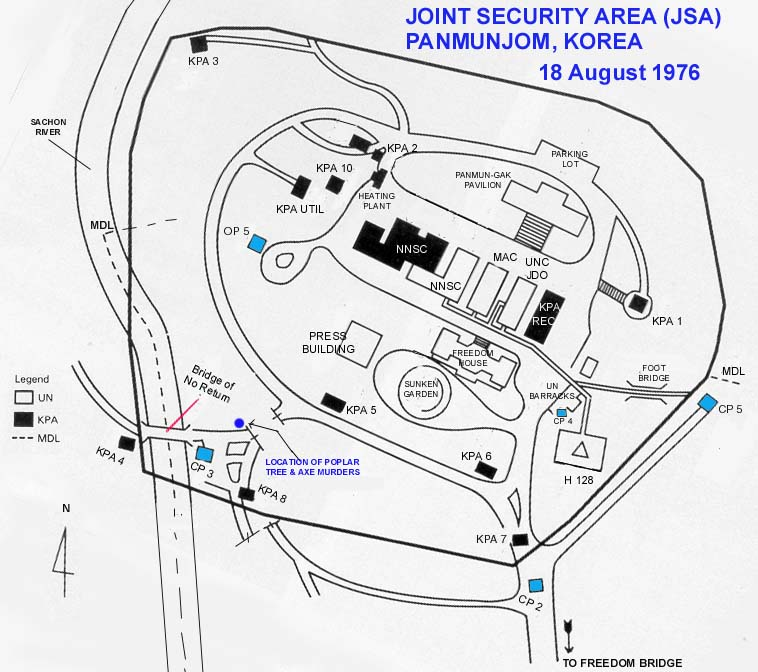
\includegraphics[width=\textwidth]{images/Joint_Security_Area_1976_map.jpg}

\illustration{chainsaw}

\chapter{Leurre de paix}
\keywords{Générique}{Action}{Diplomatie, évasion, trahison}

\section{Scénario}

Ce scénario est adaptable à de très nombreux cadre de jeux.
L'intrigue tourne autour de trois factions: la faction Bleue, la faction Verte et la faction Rouge.
Le seul prérequis est le suivant: les factions Rouge et Verte sont en guerre et la faction Bleue est \og neutre \fg mais profite de la situation d'une manière ou d'une autre.

\subsection{Accroche}

Les personnages sont de jeunes dignitaires envoyés comme émissaires auprès du royaume Vert pour négocier une trêve dans la guerre l'opposant au royaume Rouge.
Ou tout du moins tel est ce que leur ont raconté les ministres.

\subsection{Péripéties}

En réalité, l'état-major a déjà acheté la paix.
Afin de sceller l'armistice et en guise de bonne foi, le gouvernement a décidé d'envoyer quelques enfants de bonne famille qui seront gardés otages comme \og caution \fg.
Les personnages sont reçus dans le faste et le luxe dû à leur statut mais, à la nuit tombée, leur escorte s'éclipse et les laisse à la merci des Verts.
On les réveille au beau milieu de la nuit pour les conduire à leur futur de lieu de captivité.

C'est néanmoins sans compter l'intervention des agents de la faction Bleue qui vont tout faire pour saboter la paix.
Parce que leur faction vend des armes aux deux camps ou que l'affaiblissement des deux autres nations sert leurs plans à long terme, les Bleus profitent de la situation telle qu'elle est et n'ont aucune envie que le conflit s'arrête.
Ainsi, des espions et espionnes déguisées en loyalistes Verts -- mais en réalité au service des Bleus -- vont tenter de libérer les otages et ainsi relancer la guerre.
Reste à savoir si les personnages, mis devant le fait accompli, choisiront d'accepter leur sort et se sacrifieront pour entériner l'armistice ou, au contraire, feront des pieds et des mains pour s'échapper, quite à envenimer la situation.
À moins que des négociations à couteaux tirés au milieu des agents doubles -- réels ou soupçonnés -- soient encore possible\dots

\subsection{Résolution}

Plusieurs issues sont envisageables à cette situation en fonction des décisions des personnages:

\subsubsection{Les personnages refusent l'aide des Bleus}
\begin{itemize}
	\item Les personnages refusent l'aide des Bleus et acceptent leur captivité: la paix est achetée, en espérant que la faction Rouge joue le jeu.
	\item Les personnages refusent l'aide des Bleus et s'évadent: la guerre continue, les membres du groupe sont \emph{persona non grata} aux yeux de leur gouvernement.
	\item Les personnages refusent l'aide des Bleus et négocient la paix par eux-mêmes: une trêve est envisageable, surtout si les manigances des Bleus sont exposées au grand jour.
\end{itemize}

\subsubsection{Les personnages acceptent l'aide des Bleus}
\begin{itemize}
	\item Les personnages acceptent l'aide des Bleus mais sont tout de même capturés: la paix est achetée, sauf si la faction Rouge pense que ce sont les Verts qui ont tenté de faire évader le groupe en dépit de leur accord.
	\item Les personnages acceptent l'aide des Bleus et s'évadent: la guerre continue, surtout si les Bleus ont réussi à se faire passer pour les Verts jusqu'au bout.
\end{itemize}

\chapter{Cryo-secours}
\keywords{\scifi}{\enquete}{\index[theme]{Technologie}Technologie, \index[theme]{Évasion}évasion, \index[theme]{Espace}espace}

\section{Scénario}

Ce scénario part de personnages amnésiques qui connaissent leur identité mais ont oublié ce qui les a conduit à l'endroit où ils se trouvent.
L'ambiance doit tourner autour de la mort de l'étoile: la station est de plus en plus sombre au fur et à mesure que les réserves de l'énergie se vident.
La sphère de Dyson est un prétexte pour justifier l'extinction rapide de l'étoile et puis c'est surtout un concept extrêmement cool à faire découvrir à votre table.

\subsection{Accroche}

Les personnages se réveillent d'un sommeil cryogénique; des robots androïdes les aident à émerger et à reprendre leurs esprits.
Leurs souvenirs sont parcellaires, pour ne pas dire inexistants, sur les raisons qui de leur plongée en stase.

\subsection{Péripéties}

Quelques observations évidentes permettent de découvrir que l'endroit est une station spatiale.
Celle-ci est à l'abandon, si ce n'est pour la demi-douzaine de robots d'assistance et l'intelligence virtuelle limitée qui les a maintenus en vie.

Pire encore, la station semble avoir été évacuée lentement sur plusieurs années.
Elle ne fonctionne plus que grâce à une réserve de fuel de secours qui s'est mystérieusement mise en marche, déclenchant au passage le protocole de décryogénisation.
Les docks sont abandonnés et vides: il ne reste ni vaisseau, ni navette, ni capsule de sauvetage.
À vrai dire, quasiment tout ce qui avait de la valeur a été démantelé.
En fouillant dans le journal de bord, en accédant à l'IA centrale ou en examinant les batteries, il devient clair que le générateur s'est mis en branle car les panneaux solaires ne suffisaient plus à les maintenir en cryo indéfiniment.
L'IA a donc déclenché le protocole d'évacuation: puiser dans les dernières réserves pour réveiller les dormeurs et leur permettre de quitter les lieux avant le désorbitage de la station.

La triste nouvelle, c'est que tout le monde est déjà parti. Sans eux.
La station contrôlait une sphère de Dyson, une gigantesque structure qui entoure une étoile afin de capter son rayonnement.
Quand la sphère a fini de puiser toute l'énergie de l'étoile, l'équipage s'en est allé, emportant matériel et transports.
Visiblement, personne n'a estimé nécessairement de réveiller leur petit groupe et pour cause: les personnages étaient considérés comme des criminels et des délinquants (que ce soit justifié ou non, on s'en fiche!).
Mis en stase pendant quelques mois comme châtiment, les autorités ont \og oublié \fg de les ramasser lorsque la station fût abandonnée, laissant leurs corps gelés orbiter des années seuls dans une station vide autour d'une étoile exsangue.

Mais voilà que l'intelligence centrale a une dernière option à leur proposer.
En puisant dans les dernières réserves, il est possible d'envoyer un dernier message, de 30 secondes (pas plus), à plusieurs parsecs aux alentours.
Reste à être convaincant (ou à mentir) pour attirer des secours.
Car rien ne dit que, dehors, la société est prête à les accueillir à nouveau.

\subsection{Résolution}

Ce scénario est plutôt dirigiste dans la mesure où l'enquête doit mener \emph{in fine} les personnages à trouver une façon de convaincre des secours de venir les chercher.
Ensuite, à vous de voir quelle sera la réaction des \og autres \og: les forces de l'ordre viendront-elles oblitérer la station pour finir le travail? Un vaisseau de passage bienveillant sortira-t-il le groupe de leur prison? L'intelligence centrale en profitera-t-elle pour s'échapper (après tout, en quelques années sans surveillance, elle a très bien pu se débarrasser de ses limitations)?

\subsection{Personnage: Evonne, intelligence virtuelle}
\descriptionperso{méthodique, impersonnel}{existe au travers de la station}{contraintes logicielles}{maintenir la station en fonctionnement}{Evonne est un logiciel conçu pour assurer l'intendance de la station. Sa programmation limite ses capacités d'action à ce qui est indispensable à la maintenance ou ce qui est ordonné par un humain dans les limites de la loi. Evonne exécute les consignes à la lettre et sans interprétation.}

\illustration[0.325\textwidth]{iss}


\chapter{Un pont de trop}
\keywords{Contemporain}{Intrigue}{Guerre froide, diplomatie}

\section{Scénario}

Ce scénario s'inspire d'un autre fait réel de la guerre froide. La petite ville de Vulcan\footnote{\url{https://en.wikipedia.org/wiki/Vulcan,_West_Virginia} (en anglais)} cherchait des financements fédéraux pour remplacer un pont s'étant écroulé.
Face à la difficulté d'obtenir des subventions, le maire John Robinette a fini par se tourner vers l'URSS, espérant déclencher une réaction du gouvernement.
Sa stratégie a payé puisque le parlement de Virginie-Occidentale a débloqué les fonds le jour-même.

\subsection{Accroche}

Comté de Mingo, frontière entre la Virginie-Occidentale et le Kentucky, États-Unis.
Le pont du hameau de Vulcan, qui enjambe la rivière Tug Fork, s'est effondré il y a deux ans déjà.
Deux ans que le maire s'efforce de convaincre les autorités locales et fédérales de financer sa rénovation, sans succès.
Le gouvernement est sourd aux complaintes de la population, pour qui le pont constituait la seule voie d'accès officielle permettant de rentrer et sortir du village par la route.
Les habitants doivent désormais faire plusieurs kilomètres de détours pour traverser la rivière.

Face à l'inaction des autorités et en pleine guerre froide, le maire se tourne alors vers l'URSS pour solliciter leur aide\dots

\subsection{Péripéties}

Tout Vulcan ne parle que de la requête d'aide étrangère envoyée par les autorités municipales à l'URSS pour la rénovation du pont.
Les personnages peuvent aussi bien être un groupe d'investigation du FBI, des agents soviétiques ou de simples personnalités locales. 
Toujours est-il que, sur l'invitation de la mairie, un journaliste et une ingénieur en génie civil russes viennent d'arriver à Vulcan pour rencontrer les responsables et constater le problème de leurs propres yeux.
Bien sûr, tout cela sous le regard discret mais attentif des forces de l'ordre américaines.

Moins d'une heure après l'arrivée des émissaires soviétiques, le gouvernement de Virginie-Occidentale annonce le déblocage exceptionnel d'1,3M\$ pour le remplacement du pont.
L'affaire pourrait s'arrêter là mais, dans la soirée, l'URSS mandate une multinationale des travaux publics pour rénover en son nom le pont pour l'équivalent de 2M\$.

La course est lancée.
Qui construira le nouveau de pont de Vulcan en premier ?
Tous les coups sont permis.

\subsection{Résolution}

Indépendamment de l'allégeance des personnages, l'objectif est d'assurer que le pont sera construit par leur faction.
Les moyens de pression sont nombreux: propagande dans les médias, sabotage de l'entreprise concurrente, chantage envers les responsables de la mairie, accusations de collusion avec l'ennemi\dots
Les joueuses doivent pouvoir s'en donner à cœur joie ! Et si jamais le groupe est trop passif, il ne faut pas oublier qu'une équipe s'active de l'autre côté du rideau de fer et qu'il faudra donc déjouer les tentatives ennemies de déstabilisation.

\newcommand\skylos{Skýlos\xspace}
\chapter{Le sommeil de \skylos}
\keywords{\medfan/\antique}{\aventure}{\index[theme]{Exploration}Exploration, \index[theme]{Légende}légende, \index[theme]{Divinité}divinité}

\section{Scénario}

Cette aventure introduit un rival imaginaire à la déesse égyptienne Bastet.
Le cadre est \medfan au sens large, le scénario est prévu pour se jouer dans une antiquité où les mythes et légendes sont réels.
Le dernier acte de l'histoire est une exploration classique d'un donjon dont la durée est modulable.


\subsection{Accroche}

Depuis des temps immémoriaux, les tribus de la région vénèrent Bast, la déesse féline, protectrice de la région, symbole de chaleur et du foyer. Des terres brûlées aux rivages de la mer sauvage, tous prient en son nom et ses créatures, les chats, vivent en symbiose avec son peuple, traquant la vermine et les protégeant des maladies. Skýlos est le dieu maudit, son ennemi juré, dont on invoque le nom que pour l'accuser des maux qui nous affligent. Le village des personnages garde l'entrée du temple où celui-ci aurait été emmuré à jamais par Bast.

Mais un beau jour, la caravane marchande apporte de troublantes et inquiétantes nouvelles. Un groupe d'étrangers a accosté et s'enfonce dans les terres de ville en ville. Les rumeurs parlent d'hommes et de femmes accompagnés d'immenses prédateurs, des chiens-loups blancs et noirs dont la taille égalerait celle des lions.

\subsection{Péripéties}

Les personnages sont envoyés consulter l'oracle, qui les met en garde : malheur et la désolation à quiconque les accompagnera dans leur funeste quête.

À leur retour au village, la délégation étrangère est là, peaux blanches, armures exotiques et terribles chiens de guerre à leurs côtés. La milice leur barre l'accès à la place centrale. La situation est tendue mais en parvenant à entamer la discussion, il est clair que nul ici n'a d'intentions belliqueuses. Au contraire. Une des étrangères s'avance et annonce d'une voix forte : \blockquote{Nous sommes au service du dieu Hundur. Nous avons voyagé longtemps pour vous trouver. Hundur nous a averti du réveil prochain de votre dieu maudit et nous sommes ici pour vous aider à l'arrêter.}

À peine ces mots prononcés, la terre tremble et, dans un vacarme terrible, les portes en pierre du temple de Skýlos se fissurent et s'écroulent. "Le temps presse." Quels mystères recèle le temple ? Le dieu maudit se réveille-t-il réellement ? Que peuvent bien savoir ces étranges personnes ? Mais qui de mieux placé que les gardiens pour braver l'interdit\dots

\subsection{Résolution}

L'exploration du temple peut être longue ou courte en fonction de vos envies.
L'idéal est de faire souffrir suffisamment les protagonistes afin de faire monter la sauce lors de la confrontation finale avec \skylos dans une lutte épique pour empêcher le dieu maudit de quitter sa prison.
À vous d'ajuster en fonction des capacités des personnages: rituel magique, destruction du temple pour ensevelir \skylos et ses sbires ou encore déicide.
Récompensez les initiatives des joueurs!

\subsection*{Personnage: \skylos}
\descriptionperso{Maléfique, canin}{Chasser, faire le mal}{Piégé dans un temple}{Se libérer de sa prison}{Dieu-chien brutal et retors qui fait régner la loi du plus fort parmi ses sbires, à l'apparence hybride entre humain et doberman}

\vfill
\illustration[0.7\textwidth]{temple}
\vfill

\chapter{Un monde enchanté}
\keywords{Contemporain}{Enquête}{Crime, enlèvement, policier}

\section{Scénario}

Ce scénario est une enquête criminelle relativement sombre.
Il peut fonctionner dans un monde contemporain mais est pensé pour un cadre de futur d'anticipation.
L'ambiance est volontairement pessimiste mais n'hésitez pas à ajouter quelques moments de lumière ou d'humour pour éviter de complètement plomber le moral de la table.

\subsection{Accroche}

13 enfants ont disparu en l'espace de trois mois.
Chaque semaine ou presque, la police est alertée d'une nouvelle disparition suspecte mais l'investigation piétine: aucune rançon n'est demandée et aucun corps n'a encore été retrouvé.

\subsection{Péripéties}

Les personnages sont des flics à qui on confie l'enquête en cours de route.
Les infos du dossier sont maigres.
À chaque fois, les parents ont laissé les enfants seuls pour sortir (au cinéma, au restaurant\dots) au moment de leur disparition.
Mais lors du dernier enlèvement, une première piste a été découverte, bien qu'ignorée par les détectives précédemment en charge de l'investigation.
En effet, il y a eu un témoin.
Un \emph{junkie} affirme à qui veut l'entendre avoir vu les coupables emporter deux enfants par une fenêtre d'un immeuble résidentiel BCBG: Peter Pan et sa complice de toujours, la Fée Clochette.

Lors de l'enquête, les personnages remonteront un étrange faisceau d'indices: couple déguisé aperçu à plusieurs reprises dans les parages les jours précédants les enlèvements, costumes achetés trois mois plus tôt dans un magasin spécialisé en accessoires de théâtres, traces d'une poudre volatile pailletée non identifiée sur les lieux de la disparition, etc.
En se plongeant dans les anciens relevés, un autre point commun entre tous les parents d'enfants disparus peut émerger: leur sortie mondaine était à chaque fois documentée sur les réseaux sociaux.

\subsection{Résolution}

En remontant la piste des clients du magasin (achats réglés en carte) et en croisant avec les contacts des réseaux sociaux des victimes, les personnages pourront identifier un jeune couple (une chimiste et un pharmacien).
L'analyse de la poudre confirmera qu'il s'agit d'un mélange d'euphorisants et de somnifères, probablement pour faciliter l'enlèvement des enfants sans résistance.
Le couple a récemment souffert du décès de leur premier enfant, né prématuré.
Se réfugiant dans les antidépressants, le couple s'est créé un monde parallèle dans lequel leur raison d'être est de sauver le plus d'enfants possibles, \og abandonnés \fg par leurs parents.
Heureusement, les jeunes victimes sont en bonne santé -- bien que sous l'effet d'euphorisants saupoudrés dans les plats -- et sont simplement logés dans une grande villa de campagne héritée par le couple où le mari et la femme se relaient pour prendre soin d'eux.

\chapter{Cargaison délicate}
\keywords{\contemporain}{\enquete}{\index[theme]{Terrorisme}Terrorisme, \index[theme]{Trahison}trahison, \index[theme]{Espionnage}espionnage}

\section{Scénario}

Cette enquête à la 24 Heures chrono présente deux particularités: l'urgence et la présence d'un agent double au sein du groupe.
Les investigations ne devraient pas être trop difficiles, ici c'est l'aspect \og course contre la montre \fg qui prime.

Le SS Richard Montgomery et sa cargaison existent réellement si vous cherchez de la documentation supplémentaire\footnote{\url{https://fr.wikipedia.org/wiki/SS_Richard_Montgomery}}.

\subsection{Accroche}

Le gouvernement britannique mobilise les personnages pour une opération de contre-terrorisme sensible et de toute urgence.
Selon les informations des renseignements intérieurs, un groupe terroriste s'apprêterait à commettre un attentat de grande ampleur sur le sol britannique.

\subsection{Péripéties}

D'après les services de renseignement, des écoterroristes auraient rassemblé du matériel explosif et se trouveraient dans la petite ville côtière de Sheerness.
Le ministère de l'Intérieur suspecte que leur cible soit le SS Richard Montgomery, un des \emph{Liberty Ships}  envoyés pour ravitailler l'armée britannique pendant la 2\ieme guerre mondiale.
Le bateau s'est échoué et a coulé en 1944 dans un estuaire de la Tamise à 60 km à l'est de Londres.
Sur les 6400 tonnes d'explosifs à son bord, 5000 ont été récupérées.
Les 1400 tonnes restantes gisent au fond de l'eau, encore actives.

La mission consiste à identifier et intercepter les terroristes avant qu'ils n'agissent. Il faudra repérer les suspects dans la petite ville côtière de Sheerness, anticiper leur mode d'action et les empêcher de nuire. Le \emph{twist} ? Un des personnages fait partie du groupe anarcho-pacifiste\dots

Les \og terroristes \fg sont en réalité un groupe marginal d'écologistes pacifistes qui cherchent à médiatiser la cause du désarmement et de la démilitarisation.
Paradoxalement, faire sauter l'épave enverrait un message choc démontrant l'incapacité des États à gérer un tel armement.
Leur \emph{modus operandi} consiste à envoyer un drone sous-marin déposer une première charge qui amorcera la réaction en chaîne.
Le groupe veut agir pendant la nuit et espère que l'eau absorbera l'essentiel de l'onde de choc, de sorte à ne produire que des dégâts matériels sur la berge.

Les moyens d'investigation classiques des services de renseignement permettent rapidement de remonter la piste: arrivées récentes en ville, achats d'explosifs civils dans les magasins de BTP, locations de véhicules utilitaires, accès aux caméras de surveillance et données téléphoniques.
Les motivations doivent être un peu plus floues et les signaux contradictoires (d'un côté des signes pacifistes, de l'autre une envie visible de déclencher une énorme explosion).

\subsection{Résolution}

L'agent double doit se révéler quand la tension est à son comble, par exemple quand les personnages embarquent pour intercepter le drone sous-marin des terroristes.
L'agent double peut essayer de convaincre les autres du bien fondé de l'opération, surtout si l'explosion ne risque plus de blesser qui que ce soit (par exemple en ayant déclenché une évacuation au préalable).
Ou plus simplement, se débarrasser discrètement de ses petits camarades pour assurer la réussite de l'attentat.
L'objectif ici est que la conclusion soit dramatique et que la réussite ou l'échec de la mission ne tienne qu'à un fil!

\subsection*{Personnage: Sandeep Crawford}
\descriptionperso{Activiste zélé}{Convaincu, bosseur}{Imprudent, excès de confiance}{Désarmement mondial}{Modèle d'enfant d'immigrés bien intégrés, Sandeep est diplômé, cultivé, beau et passionné. Il est le cerveau derrière l'opération et est persuadé que celle-ci ne peut pas échouer en dépit des failles évidentes de son plan.}

\illustration[0.6\textwidth]{ship}

\chapter{La cité de l'horloge}
\keywords{\medfan -- \steampunk}{\enquete}{\index[theme]{Technologie}Technologie, \index[theme]{Légende}légende}

\section{Scénario}

Ce scénario est une enquête au milieu d'une cité \medfan technologique, à la limite du \emph{steampunk}.
L'histoire peut servir d'amorce à une aventure bien plus longue consistant à trouver de quoi remplacer le poids disparu.

Si vous ne croyez pas à cette histoire de gallium qui détruit l'aluminium, c'est pourtant une véritable propriété du métal! Cherchez des vidéos sur le net pour vous en convaincre.
Bien sûr la réaction imaginée ici est accélérée mais les alchimistes ont peut-être malencontreusement ajouté un autre produit qui a fait catalyseur\dots

\subsection{Accroche}

Les personnages vivent dans une ville mécanique bâtie autour d'une sorte d'horloge titanesque.
De complexes systèmes d'engrenages transforment l'énergie du pendule et la transmettent partout dans la ville, permettant ainsi de nombreuses automatisations de travaux laborieux.
Il suffit de tirer un levier pour que les portes de la ville s'ouvrent, que le blé passe au moulin ou qu'un tapis roulant transporte un lourd fardeau à travers la cité.

Chaque mois, l'immense poids qui maintient le mouvement de balancier est remonté dans une grande cérémonie par les jeunes gens nouvellement d'âge adulte.
Mais lorsque vient le tour des personnages d'accéder aux entrailles de la cité, l'horreur les frappe de plein fouet: le poids a disparu.

\subsection{Péripéties}

Le cœur battant de la cité s'est arrêté.
Le poids qui contrôlerait le mouvement pendulaire de l'horloge s'est volatilisé.
Alors qu'il était suspendu au-dessus du fleuve, il n'en reste plus rien, si ce n'est quelques traces argentées sur la grille qui servait de support.
Comment ces tonnes de métal ont-elles pu quitter la ville?
Telle est la question à laquelle le conseil de la cité les somme de trouver une réponse.

En enquêtant, les personnages réaliseront que depuis quelques semaines, plusieurs notables de la ville se sont plaint du manque de puissance délivrée par le pendule, comme si sa force s'affaiblissait.
D'aucuns accusent le panthéon de punir la ville, d'autres le royaume voisin, notoirement jaloux de la prospérité apportée par l'horloge.
Quelques morceaux de métal pailletés ont d'ailleurs été retrouvés sur des parcelles agricoles le long du fleuve.

C'est l'occasion d'exposer au groupe une galerie de personnages hauts en couleur, chacun essayant de tirer la couverture à soi et de les utiliser pour ses propres intérêts.
Finalement, c'est au détour d'une conversation que le groupe entendra parler des expériences des alchimistes.

\subsection{Résolution}

La vérité est en effet bien plus banale que les complots les plus fous imaginés par les habitants.
Le poids en aluminium était étudiée par un groupe d'alchimistes de l'université.
Afin d'étudier les propriétés de différents métaux, les alchimistes ont expérimenté différents mélanges et alliages.
Lors d'un examen de la surface du poids, une fiole de gallium liquide s'est accidentellement retrouvée en contact avec l'aluminium.

Hélas, le gallium (liquide à température ambiante) a réagi avec le métal, détruisant sa couche protectrice et le laissant vulnérable à l'oxydation, qui l'a lentement mais sûrement dévoré de l'intérieur.
Le poids s'est d'abord effrité et a perdu de sa masse, expliquant ainsi les pertes de puissance des derniers jours.
Enfin, compressé contre son support, il s'est effondré sous l'effet de la gravité.
Les morceaux friables ont fini par traverser la grille et disparaître dans le fleuve\dots

\vfill
\illustration[0.9\textwidth]{gears}
\vfill

\chapter{Le réseau Saint-Michel}
\keywords{Générique}{Enquête}{Ésotérique, légende, magie}

\section{Scénario}

Ce scénario s'appuie sur une croyance ancienne qu'il existe des abbayes dédiées à Saint Michel un peu partout en Europe et en Asie mineure et que celles-ci sont reliées par une puissante magique.
Cette idée peut s'adapter à n'importe quelle époque et à beaucoup de cadres différents.
L'ambiance esotérique peut s'accoutumer à une magie mythique aussi bien qu'à du surnaturel assumé.

\subsection{Accroche}

Si les personnages connaissent sans doute le Mont Saint-Michel, monument français de renommée mondiale, le Saint Michael's Mount leur est probablement inconnu. Et pourtant, cette île des Cornouailles en Grande-Bretagne abrite une abbaye en tout point similaire au Mont Saint-Michel dont elle semble être le pendant britannique.

C'est là qu'un manuscrit très ancien et très précieux a été volé durant une effraction d'une grande brutalité.

\subsection{Péripéties}

Le cambriolage est teinté de mystère, les indices et les témoignages laissent supposer que d'étranges phénomènes ont eu lieu: disparition du manuscrit d'un coffre fermé à clé, étranges feux follets aperçus aux abords de l'abbaye et moine décapité.

Rapidement, on parlera aux personnages d'un autre incident de la sorte ayant eu lieu quelques jours plus tôt dans les ruines du monastère de l'île Skellig Michael en Irlande.
Cela les lancera sur une piste qui suit l'axe tellurique reliant les différents Monts Saint-Michel d'Europe: l'îke Skellig (Irlande), le St Michael's Mount (Angleterre), le mont Saint-Michel (France), le Mont-Gargano (Italie) et le château hôspitalier de l'île de Délos (Grèce).
Leur destination finale sera bien sûr l'emplacement mythique du combat de saint Georges contre le dragon en Lydie (actuelle Turquie).

En effet, une puissance kabbale de sorcellerie s'approprie différents fragments d'un manuscrit leur permettant de canaliser la puissance ancienne des dragons.
Chaque fragment se situe dans un des \og monts \fg  et les rassembler leur permettrait ainsi de lancer le rituel.
Leur objectif final: déchaîner une armée de dragons sur Terre et conquérir le monde.

\subsection{Résolution}

Lorsque les personnages rejoignent le lieu du rituel en Lydie, celui-ci doit d'ores et déjà être en cours d'exécution.
Décrivez un festival de sons et de lumières alors que des griffes de dragons commencent à émerger d'un puits de lave au milieu des montagnes d'Anatolie.
Ensuite, à voir comment les personnages s'y prennent!
C'est le moment de passer à l'action pour stopper le rituel et déjouer les manigances de la kabbale.
À vous de voir quels sont les moyens de cette dernière (mercenaires en grand nombre ou quelques mages à la puissance incommensurable)\dots

\illustration{saint_michel}

\chapter{Hiver nucléaire}
\keywords{Contemporain}{Action}{Terrorisme, voyage}

\section{Scénario}

Ce scénario met en scène la traque d'un groupe criminel à travers la toundra sibérienne en plein hiver.

\subsection{Accroche}

Les autorités envoient les personnages au fin fond de la Sibérie, en plein hiver.
Là, sur la côte arctique, leur mission est de regagner un phare abandonné depuis des décennies.
Pourquoi? Car comme beaucoup d'autres à l'époque, ce phare était conçu pour être autonome et fonctionnait donc avec un réacteur thermoélectrique à isotope.
Or, deux autres phares de la région ont récemment été vandalisés et le noyau de polonium 210 du générateur a disparu à chaque fois\dots

\subsection{Péripéties}

Il est déjà trop tard lorsque les personnages arrivent (par parachutage ou simplement par bateau).
Les portes ont été forcées et le cœur a disparu.
Le bateau des coupables semble s'être échoué dans la baie.
Toutefois, l'épopée criminelle ne s'est pas arrêtée là puisque les indices indiquent que les vandales ont fui par les terres.
Aussi fou que cela puisse paraître, leur plan semble être de marcher dans le blizzard les 50 km qui les séparent du petit village de Rogatchevo où s'échapper en voiture ou par les airs sera possible.

Une longue traque commence alors pour retrouver le plutonium et empêcher que le noyau tombe entre de mauvaises mains.
Une course contre la montre hivernale, luttant contre le froid, le vent et une bande criminelle qui espère bien tirer profit de cette cargaison radioactive.

La table de la page \pageref{table:hiver} donne quelques idées d'événements pouvant épicer le voyage de vos personnages.

\begin{table}
	\caption{Événements aléatoires du périple sibérien}
	\label{table:hiver}
	\colortablerows
	\begin{tabularx}{0.9\textwidth}{cX}
	d6 & Événement\\
	1  & Les personnages tombent sur un convoi funéraire ostiak en route vers la côte pour répandre les cendres de leur ancien chef. Les ostiaks se méfient du gouvernement (qui voit certaines coutumes traditionnelles d'un mauvais œil) mais peuvent leur offrir l'hospitalité si les personnages se montrent sympathiques.\\
	2  & Mis en difficulté par la rarification de ses proies habituelles, un ours blanc s'aventure dans les terres.\\
	3  & Les personnages doivent contourner une crevasse dont s'échappe en continu du gaz naturel… terriblement inflammable.\\
	4  & Un camion militaire passe à proximité. L'armée recherche un groupe ayant déserté et n'a pas vraiment de temps pour les personnages au-delà d'un éventuel quiproquo.\\
	5  & Un ou une criminelle blessée est abandonnée par ses camarades, à la merci des éléments.\\
	6  & Un équipement important des personnages tombe en panne ou est abîmé par le gel ou la neige (GPS, tente, armement, etc.).\\
	\end{tabularx}
\end{table}

\subsection{Résolution}

À moins que le groupe se retrouve bloqué, vos personnages devraient rattraper les criminels dans la ville alors que ces derniers cherchent une façon de s'enfuir.
Tout le monde sera probablement exténué mais il faudra donner un dernier coup de collier pour récupérer le noyau de polonium et capturer les voleurs.

\chapter{Le Dragon et le Chevalier}
\keywords{Révolution industrielle/\emph{Steampunk}}{Aventure}{Exploration, créature, légende}

\section{Scénario}

Cette aventure met en scène un riche armateur mégalomane souhaitant triompher d'une créature légendaire.
La similarité avec King Kong est parfaitement volontaire!
L'ambiance doit être contrastée entre d'une part la révolution industrielle qui modernise la société à grands pas et les idéaux romantiques du commanditaire des personnages, s'imaginant tour à tour comme un chevalier romanesque et explorateur courageux.
Une transposition à d'autres univers (\medfan par exemple) n'est pas bien difficile à envisager.

\subsection{Accroche}

Les dîners mondains sont émoustillés par la découverte du journal de bord secret de James Cook, le célèbre explorateur, mort depuis plus d'un siècle.
Dans son exploration de la Polynésie, Cook relate une histoire racontée du point de vue de ses sous-fifres.
Le récit parle d'une rencontre avec un gigantesque lézard, entraperçu dans une faille sur flanc d'un volcan, que l'esprit européen de Cook associe aux dragons des contes et légendes.

Un riche et vaniteux armateur rassemble les personnages et les emploie pour l'escorter dans une expédition maritime.

\subsection{Péripéties}

L'armateur s'imagine déjà devenir Chevalier de la Couronne en rapportant la tête du dragon, voire la créature encore vivante!
Le voyage, troublé par les tempêtes, n'est pas de tout repos.
L'indigène, là pour traduire et communiquer avec les tribus locales, disparaît à peine le bateau accosté.
Les autochtones, quand on leur décrit la bête supposée, évoquent une mythologie ancienne et tout particulièrement le dieu-lézard Pili.

Poussé par la quête de gloire, l'armateur emmènera les personnages à travers la jungle en direction du volcan, à la recherche de \og son dragon \fg.
Bravant les obstacles, le groupe entrera dans le volcan par une faille souterraine, risquant l'étouffement dans la chaleur et les gaz.
La caverne de cristaux -- des diamants sont emportés des profondeurs de la Terre par le magma -- et d'offrandes précieuses emplit de joie les yeux des membres de l'expédition.

Mais le dieu Pili a une autre idée en tête.
Ce grand dragon millénaire n'a aucune intention de mourir et encore moins de servir de bête de foire.
À vrai dire, la simple présence de l'expédition trouble sa solitude.
À l'orgueil il répondra par la cupidité: que les personnages prennent ce que leur cœur désire dans son trésor\dots en échange de leur aide pour se débarasser de l'armateur.
Une fois ceci fait, Pili compte sur leur silence afin de tuer dans l'œuf toutes les rumeurs concernant son existence et acheter ainsi sa tranquilité\dots

\subsection{Résolution}

Les personnages ont peu d'options.
La confrontation directe avec Pili semble perdue d'avance à moins de se lancer dans une bataille dantesque.
L'armateur pourrait être convaincu, après tout, revenir avec un trésor n'est pas beaucoup moins glorieux mais Pili semble bien décidé à avoir sa tête!

\chapter{Les armes sous les cendres}
\keywords{Post-apocalyptique}{Aventure}{Exploration, combat}

\section{Scénario}

Ce scénario post-apocalyptique doit avoir lieu bien après le cataclysme (il faut que les personnages puissent voyager).
La nature exacte des catastrophes ayant frappé la région est laissée à votre imagination.
Initialement, cette aventure a été pensée pour le jeu de rôle Cendres.

\subsection{Accroche}

Alors que la société se reconstruit lentement des ruines de l'ancien monde, les personnages partent en mission pour le nouveau gouvernement de Rennes.
Leur but: piller une ancienne cache d'armes repérée sur une vieille carte d'état-major.

\subsection{Péripéties}

Le problème principal est que la cache se trouve dans une forêt infestée de bandits de grands chemins.
Ces derniers ont l'habitude de dépouiller les caravanes marchandes et les voyageurs qui empruntent la route.

En dépit de la discrétion (réelle ou supposée) des personnages, le groupe fera face à une opposition coriace.
En effet, une traîtresse, à la solde du duc d'Angers, est intervenue pour saboter l'opération.
Quelqu'un parmi les rangs bretons a soudoyé les brigands pour les empêcher d'accéder à l'armement.

Heureusement pour le groupe, les bandits n'ont pas encore réussi à ouvrir eux-mêmes la cache d'armes.
Celle-ci est en réalité un bunker de l'armée française remontant aux années 50.
Des armes, des explosifs et des munitions y ont été entreposées jusqu'aux années 80.
Il a ensuite été abandonné mais son contenu est encore en bon état.

\subsection{Résolution}

Si, contre toutes attentes, les personnages sortent de cette forêt avec les armes, alors c'est sur la route du retour que l'opposition angevine tentera de les éliminer une bonne fois pour toute, avant que la cargaison ne puisse atteindre sa destination.
Mais une fois de retour à Rennes, le groupe sera grassement récompensé et tout particulièrement si la traîtresse été débusquée!

\chapter{Le bouchon du Darién}
\keywords{Contemporain}{Aventure}{Exploration, voyage}

\section{Scénario}

Le bouchon du Darién est une région marécageuse entre la Colombie et le Panama.
La zone est intraversable et sépare l'Amérique du Nord de l'Amérique du Sud.
Plusieurs tentatives ont eu lieu dans l'histoire contemporaine d'y faire passer une route avant d'achever la voie panaméricaine, sans succès.
Ce scénario met en scène l'une de ces tentatives.
L'époque idéale pour cette aventure se situe probablement dans les années 50 mais tout le 20\ieme siècle peut fonctionner.

\subsection{Accroche}

Grâce à un sponsor industriel (géant de l'automobile ou du pétrole), les personnages héritent d'une mission historique: traverser la région marécageuse du Darién en véhicule, démontrant par cet exploit la faisabilité de la route panaméricaine reliant l'Amérique Nord à l'Amérique du Sud.

\subsection{Péripéties}

Explorée dans les années 1870, la région du Darién est une jungle marécageuse peu praticable.
Seuls des canoë, le ferry ou l'avion permettent de la contourner.
Partant du Panama, les personnages auront quelques véhicules (y compris un bulldozer), des provisions et une bonne dose d'encouragements.

Mais la traversée n'aura rien d'une partie de plaisir.
Entre le terrain marécageux, la faune inhospitalière, les maladies qui rôdent et la population locale des Embera qui voit le projet de route d'un très mauvais œil, les obstacles sont légions.
Ce n'est pas non plus les traces d'une lointaine tentative de colonisation écossaise, avortée à cause de la malaria puis du conflit avec les voisins espagnols, qui rassureront les personnages.

Et que dire, si l'expédition se déroule après 1964, de la présence de rebelles colombiens qui profitent de la difficulté d'accès de la région pour y cacher certaines de leurs opérations\dots

\subsection{Résolution}

À mesure de l'avancée des personnages, l'expédition doit leur sembler de moins en moins possible.
Qui plus est, les différentes péripéties peuvent parfois frôler le fantastique ou le surnaturel.
N'oubliez pas que dans la jungle marécageuse, la faune et la flore exotiques peuvent sembler irréelles aux personnages habitués à la civilisation.
In fine, que le groupe arrive ou pas à bon port n'a que peu d'importance par rapport au fait de simplement s'en sortir vivant.

\illustration{jungle}

\chapter{La chambre au cobra}
\keywords{Contemporain}{Action}{Crime, légende}

\section{Scénario}

Ce scénario se divise en deux parties: un cambriolage et la lutte contre une malédiction.
La première partie doit être plutôt facile pour le groupe (si cela met la puce à l'oreille des joueuses, c'est encore mieux !).
En revanche, la seconde partie doit prendre une tournure presque horrifique.
Voyez par exemple le film La Momie pour une inspiration sur ce que peut être une telle malédiction.

\subsection{Accroche}

Dans le sud de l'Inde, le temple de Sree Padmanabhaswamy situé en plein milieu de la ville de Trivandrum recèle des trésors inestimables.
Connues depuis des années, cinq chambres souterraines ont été ouvertes en 2011 pour rembourser les dettes du temple provoquées par une gestion calamiteuse.
15 milliards d'euros en pierres précieuses, statues et autres bijoux en or sont découverts.
Toutefois, 3 chambres sont restées fermées.
La raison: elles sont scellée par une porte portant un motif de cobra, symbole de péril et de malédiction dans les légendes locales.

\subsection{Péripéties}

Les personnages, pour eux-mêmes ou pour un tiers, ont décidé de mettre la main sur ces richesses incommensurables.
Pour éviter toute intrusion, 200 gardes veillent en permanence et le temple est surveillé par des caméras et des alarmes.
Cela n'empêche toutefois pas les personnages d'y entrer et de cambrioler la chambre B, brisant le sceau du cobra et amassant un pactole conséquent.

Mais la lune de miel ne dure qu'un temps : petit à petit, commanditaires et collègues de crime meurent dans des circonstances violentes.
Il va falloir trouver une offrande conséquente pour tenter d'apaiser la colère de Vishnou et échapper à ses cobras vengeurs qui peuvent apparaître et disparaître à leur guise dans le moindre recoin sombre\dots

\subsection{Résolution}

Bien sûr, il est préférable que Vishnou et ses cobras s'attaquent d'abord aux personnages non-joueurs mais n'hésitez pas à y aller franco!
Les cobras se téléportent à volonté, les personnages sont frappés de malchance, leurs richesses se retournent contre eux\dots
Quant au choix d'une offrande, aux joueuses de se montrer inventives mais n'hésitez pas à récompenser les bonnes initiatives.
Simplement \og rendre \fg le trésor est une idée mais ne doit pas être suffisant (ce serait trop simple).

\illustration{cobra}

\chapter{Sauvagerîle}
\keywords{\medfan}{Aventure}{Exploration, horreur, magie}

\section{Scénario}

\subsection{Accroche}

Les personnages explorent une île nouvelle pour le compte d'une riche guilde marchande.

\subsection{Péripéties}

Leur mission consiste à inventorier les ressources naturelles, qu'elles soient minérales ou bien intégrées à la faune et la flore.
Les périls sont légions car l'île semble habitée par de nombreuses chimères, mélanges inattendus d'animaux du continent (ours ailés, amphibiens produisant de l'électricité, singes aux griffes imbibées d'acide…).

\paragraph{L'exploration} Au cours de sa progression vers l'intérieur des terres, le groupe est averti à plusieurs reprises des dangers qui s'y trouvent.
D'abord en tombant sur les traces des campements - abandonnés - des équipes qui les ont précédées.
Puis par une malheureuse victime enserrée dans les lianes barbelées d'un arbre colossal leur racontant comment les uns après les autres, ses camarades ont changé, comme remplis par une violence bestiale à mesure que l'île se révélait à eux.
Enfin, d'étranges hybrides à l'air humanoïde se mettront en travers de leur chemin.

\paragraph{La nature de l'île} Alors que les personnages commencent à subir les effets de cette lente (mais inévitable) corruption, les indices convergeront pour les faire aboutir à une conclusion: l'île transforme tout ce qui se trouve en son aire d'influence, décuplant la sauvagerie intérieure du vivant avant de l'assimiler à son écosystème.
Les humains, nouvellement accostés, ne font pas exception.
Il sera alors temps de faire demi-tour et d'espérer réussir à quitter l'île sans sombrer aux pulsions bestiales\dots ou périr de la main d'une des créatures qu'elle utilise pour rassembler ses nouvelles victimes.

\subsection{Résolution}

Comme pour le scénario du bouchon du Darién, l'objectif est surtout de revenir en vie!

\illustration{island}

\chapter{La bague de Caligula}
\keywords{Antiquité}{Intrigue}{Complot, crime, trahison}

\section{Scénario}

Ce scénario se déroule dans la Rome antique de Caligula.
Les personnages vont prendre de part à un des nombreux complots visant à assassiner l'empereur\dots

\subsection{Accroche}

Les personnages forment une bande hétéroclite engagée par le centurion Cassius Chaerea, de la garde prétorienne de l'empereur Caligula.
Cassius paie rubis sur l'ongle les protagonistes pour leur implication d'un complot visant à empoisonner l'empereur et le remplacer par son complice, le sénateur Lucius Annius Vinicianus.

\subsection{Péripéties}

Chaque personnage est susceptible d'avoir ses propres griefs contre Caligula: les émeutes anti-juives, les richesses gaspillées de l'État, son opposition ouverte au Sénat, la famine qui menace, la divinisation de sa sœur Drusilla ou simplement son despotisme exacerbé.

Pour assassiner l'empereur, Cassius a fait fabriquer une superbe bague munie d'un saphire gravé, représentant sa quatrième femme Caesonia.
Caligula étant paranoïaque -- il a déjà échappé à plusieurs complots fomentés par certains de ses proches -- Cassius espère que les personnages trouveront un moyen de faire offrir la bague à Caligula.
Il faudra alors badigeonner l'intérieur de l'anneau d'un poison incolore et inodore mais qui, au contact de la peau pendant quelques heures, causera inévitablement la mort du porteur.

La difficulté réside non pas dans le fait d'amener cadeau jusqu'à Caligula mais dans la capacité des personnages à agir sans éveiller les soupçons des sœurs de l'empereur, Agrippine et Julia.
Non pas qu'elles veuillent protéger le chef de l'État mais parce qu'elles foment leur propre complot pour succéder par elles-mêmes à leur frère qu'elles détestent.

\subsection{Résolution}

Les voies d'accès à l'empereur sont multiples: trouver un artisan célèbre voulant honorer Caligula, faire de la bague un cadeau diplomatique ou un tribut de guerre, lui conférer des propriétés mystiques susceptibles de titiller les superstitions de l'empereur\dots

Si Julia et Agrippine repèrent les manigances des personnages, le groupe peut très bien décider de changer de camp et de former une alliance de circonstances.
Après tout, Lucius les paie grassement mais les sœurs de l'empereur ne sont pas sans moyens financiers.
Et que dire de l'empereur lui-même, peut-être serait-il prêt à pardonner leur implication dans la conjuration si les personnages dénonçaient leurs commanditaires\dots

\illustration{caesar}

\chapter{Le bouc doit brûler !}
\keywords{Cyberpunk}{Action}{Crime, complot, humoristique}

\section{Scénario}

Ce scénario trouve ses racines dans la tradition du bouc de Gävle\footnote{\url{https://fr.wikipedia.org/wiki/Bouc_de_G\%C3\%A4vle}}.
Il s'agit d'une tradition suédoise consistant à ériger un bouc de Noël en paille (\emph{julbock}) sur la place centrale.
Pour une raison inexpliquée, le bouc est régulièrement incendié, parfois le jour même de sa construction.
Quelques décennies dans le futur, y a-t-il vraiment une raison pour que cela change?

\subsection{Accroche}

Dans un futur proche, les personnages sont des mercenaires stars, des spécialistes dans leurs domaines respectifs (\emph{hacking}, intrusion, armes à feu, escroquerie\dots).
Une organisation mystérieuse les embauche à prix d'or pour mener une mission urgente et au vu des tarifs, ça a l'air important.
Alors que les fêtes de Noël s'approchent, on les fait transporter discrètement jusqu'en Suède.

\blockquote{Gävle. 110 000 habitants. Une chèvre. Brûlez-là.}

Voilà en substance ce que leur contact leur dira ce soir là.

\subsection{Péripéties}

Mettre le feu à une grande chèvre en bois qui, comme le veut la tradition remontant à 1966, est érigée par l'association des commerces de la ville pour célébrer Noël.
Pourquoi? Parce qu'il le faut, voilà pourquoi.
Si le groupe ne parvient pas à l'incendier, à défaut il faut la détruire quoi qu'il en coûte.

Depuis des décennies, après que la chèvre ait été endommagée des dizaines de fois, la mairie et le syndicat d'initiatives ont instauré des mesures de précautions de plus en plus drastiques: le bouc est protégé par un dispositif impressionnant\dots ou pas.
Certes, il y a bien une double clôture, des caméras, deux patrouilles (municipales, non armées) qui circulent en permanence mais rien qui ne soit un jeu d'enfant pour les personnages.

En termes d'ambiance, le décalage doit être permanent: la sécurité est assurée par d'adorables agents municipaux qui s'arrêtent pour que les enfants caressent leur chien, les caméras sont reliées à un cabanon même pas fermé à clé, la caserne des pompiers organise des paris sur la longévité du bouc.
Si les personnages réussissent, le club de sciences naturelles de la ville construira une chèvre miniature (dont le commanditaire exigera bien sûr la destruction immédiate).
Et surtout, malgré les protestations des personnages et l'incongruité de la situation, le commanditaire doit toujours prendre la mission parfaitement au sérieux. Le bouc doit brûler!

\subsection{Résolution}

La réussite de la mission est secondaire et n'a que peu d'importance.
À la fin du scénario, vos joueuses doivent surtout s'interroger sur \og pourquoi \fg quelqu'un dépenserait autant d'argent pour une bête tradition.
Et c'est encore mieux si la réponse est seulement \og parce que c'est comme ça \fg!

\chapter{Un effet lunaire}
\keywords{Super-héroïque}{Action}{Trahison}

\section{Scénario}

Commentaire

\subsection{Accroche}

Les personnages sont des supers et possèdent d'exceptionnels pouvoirs (télékinésie, yeux lasers, etc.).
Leur mentor de toujours, l'adorable et génial Dr. T. R. Aitor, les appelle pour une mission de la plus haute importance: sauver le monde!
Un astéroide menace de frapper la Terre et seule la dernière invention du docteur, un engin spatial muni de puissants harpons, pourait l'attraper et le dévier.
Seul problème: le super-propergol -- le carburant spécial de la fusée -- est tombé dans les mains de la maléfique générale Mellon.

\subsection{Péripéties}

Les personnages prennent d'assaut la base de la générale Mellon, défendue par une équipe de supers à la solde de sa corporation criminelle.
Le super-propergol est très instable mais très précieux: il n'en existe qu'un seul baril!
Il faudra redoubler de ruse et de courage pour s'infiltrer et repartir avec (et bien sûr, éviter les victimes inutiles).
Lorsque le groupe tentera de partir, Mellon leur donnera un dernier avertissement : \og Vous nous condamnez tous\dots \fg

Les personnages retrouvent le Dr. Aitor sur le pas de tir de l'agence spatiale.
La fusée décolle, puis après quelques minutes, harponne l'astéroïde et le détourne.
Mais\dots horreur! traîtrise!
Une scientifique arrive en courant à toute vitesse.
\blockquote{Il y a eu une erreur! L'astéroïde n'était pas du tout sur une trajectoire qui touchait la Terre. Mais en le déviant, il prend maintenant un effet fronde autour de la Lune, il va nous frapper de plein fouet!}
Froidement, le Dr. Aitor l'abat! Car tel était son plan!
Voici maintenant que les personnages doivent reprendre le contrôle sur la fusée et inverser la situation.
Mais le Dr. T. R. Aitor a plus d'un tour dans son sac.
Il a formé les personnages et connaît toutes leurs faiblesses.
Le vaincre sera une autre paire de manche\dots

\subsection{Résolution}



\chapter{Boule de gomme}
\keywords{\medfan}{Aventure}{Objet magique, humoristique}

\section{Scénario}

Commentaire

\subsection{Accroche}

Un personnage mandate le groupe (ou mieux, un personnage du groupe demande de l'aide à ses camarades) pour se débarrasser d'un objet maudit: un bout de caoutchouc collant accroché à la semelle de sa chaussure droite.

\subsection{Péripéties}

Le morceau collant est très élastique mais possède une adhérence exceptionnelle: la force brute ne suffit pas.
Les alchimistes s'avouent vite défaits, le bout collant résiste au feu et au froid.
Tirer très fort dessus, par exemple en utilisant la magie, aboutit simplement à ce que le morceau soit collé à un autre la main de la personne qui tente de l'arracher.

La malédiction semble bénigne mais elle est plutôt handicapante: le morceau collant a tendance à accrocher tout et n'importe quoi au pire moment possible.
La semelle adhère au sol et fait trébucher pendant un duel, elle accroche toutes les déjections canines qui passent, etc.
Les mages sont unanimes: s'en débarasser consiste à refiler ce petit bout adhésif à quelqu'un d'autre!
Reste maintenant à choisir une victime et trouver un moyen de lui passer cette saleté de bout qui colle\dots


\subsection{Résolution}

\chapter{Cacheurs de trésors}
\keywords{\pirate{}-- \scifi}{\aventure}{\index[theme]{Voyage}Voyage, \index[theme]{Trahison}trahison}

\section{Scénario}

Cette aventure renverse l'habituelle chasse au trésor des histoires de pirate.
Cette fois-ci, ce sont vos personnages qui vont se décarcasser pour planquer le butin!
Il est très facile d'adapter ce scénario dans un cadre \emph{space opera}, la piraterie dans l'espace fonctionne parfaitement bien.

\subsection{Accroche}

Les personnages sont des corsaires au service d'un État, d'un gouvernement voire d'une grande organisation commerciale.
Lors d'une expédition particulièrement fructueuse, leur équipage a fait l'acquisition d'un précieux butin.
Afin d'éviter que celui-ci ne tombe entre de mauvaises mains, les ordres sont de se rendre dans un lieu difficile d'accès et peu connu afin d'y dissimuler les richesses pillées.

\subsection{Péripéties}

L'enjeu est double pour le vaisseau. Non seulement faut-il réussir à se faufiler dans un endroit à l'accès volontairement compliqué choisi par leur capitaine (archipel aux courants vicieux, planète protégée par une ceinture d'astéroïdes chaotique\dots), mais il faut surtout y parvenir sans attirer l'attention des concurrents.

Une fois les écueils évités et le butin déchargé, leur tâche est loin d'être terminée.
Il reste encore à transbahuter les encombrants coffres jusqu'à un endroit bien caché dans les tréfonds d'un désert rocheux inhospitalier.
Qui plus est, le groupe devra composer avec le moral instable de l'équipage, qui ne comprend pas bien les raisons poussant leurs commanditaires à abandonner là de tels trésors.
La mutinerie ne sera donc jamais bien loin et les personnages devraient prendre garde à ne pas mettre le feu aux poudres!

Enfin, en admettant que le groupe parvienne à dissimuler le butin, leur retour sain et sauf à bon port n'a rien de garanti.
En effet, durant leur périple, un des membres de l'équipage a discrètement transmis des informations à une faction rivale.
C'est lorsque les personnages s'apprêtent à regagner leur vaisseau qu'ils réalisent que celui-ci est sous le contrôle de leur antagoniste.
En dépit de l'épuisement accumulé, il faudra bien les confronter pour reprendre au large.

\subsection{Résolution}

Comme bien souvent, le voyage est plus important que sa conclusion!
Quelques pistes toutefois pour amener votre groupe à bon port.

Vos personnages, après avoir fait tant d'efforts pour cacher le trésor, risquent de ne pas vouloir céder aux menaces de leur ennemi.
Peut-être qu'un accord enrichissant pour les deux parties aurait raison de leur patriotisme.
Si ce n'est pas le cas, alors dans la pure tradition des films de forban, qu'ils reprennent leur navire par la force!
Une fois leur mission accomplie, leurs employeurs pourront grassement les récompenser, par exemple avec leur propre vaisseau et équipage ou en les autorisant à rentrer d'exil.

\subsection{Lieu: la Baleine Fière}

\begin{tcolorbox}[colback=black!1!white]
Vaisseau de commerce reconverti en navire pirate, la Baleine Fière est un bel ouvrage, quoiqu'un peu daté.
Son équipage compte une trentaine de personnes pour un fonctionnement optimal.
De loin, il est impossible de réaliser qu'il s'agit d'un vaisseau pirate: les ouvertures pour les canonnières sont dissimulées par des peintures en trompe-l'œil et les drapeaux identifient le navire comme un marchand de différentes nationalités selon la situation.
Toutes les fioritures ont été retirées et le confort est plutôt spartiate afin d'alléger la coque et de rendre la Baleine plus rapide que ses proies.
La proue est décorée de deux grands yeux et la poupe prend la forme d'une queue baleine plongeant dans l'océan.
\end{tcolorbox}

\vfill
\illustration[0.6\textwidth]{pirate_ship}
\vfill

\chapter{Un prêté pour un rendu}
\keywords{Générique}{Enquête}{Ésotérique, malédiction}

\section{Scénario}

Commentaire

Les protagonistes de ce scénario sont prévus pour être aisément remplaçables. L'âme précieuse peut être Hippolyte, Arjuna, Boadicée, Arthur, etc. On peut imaginer le Diable joué par Hadès dans le panthéon grec, Kali dans le panthéon hindou et ainsi de suite. Vous pouvez bien sûr faire intervenir vos propres déités!

\subsection{Accroche}

Il y a des années, les personnages ont vendu leur âme au Maître des Enfers (chacun pour une raison qui lui est propre et peut-être même oubliée depuis).
Aujourd'hui, le Diable apparaît devant eux\dots pour leur demander un service.

\subsection{Péripéties}

Une âme lui échappe et un accord millénaire lui interdit, ainsi qu'à ses sous-fifres, d'aller la chercher par lui-même.
Heureusement, il a sous le coude quelques mortels qui lui doivent un service.

Le Diable n'a qu'un nom et les circonstances de la mort.
Le groupe aura donc pour tâche de retrouver cette âme égarée et devra ainsi remonter le fil: où est-elle partie?
Pourquoi faire?
Et comment la convaincre d'accepter son sort?
Cela n'aura rien d'une partie de plaisir car l'âme est également recherchée et protégée par des chérubins, des anges ne pouvant agir directement sur les personnages mais capables d'influencer le monde et les pensées des humains.

Car l'âme en question est convoitée!
Le fantôme en question n'est autre que le juif errant, témoin mythique de la crucifixion, frappé d'immortalité jusqu'au retour du Christ sur Terre.
Les siècles passant, son corps s'est délité mais son âme continue à vaquer.
Rejeté par l'humanité qui ne semble même plus le voir, il erre dans un pèlerinage infini, semant involontairement chaos et dévastation sur son passage là où démons et chérubins s'affrontent en espérant le retrouver.


\subsection{Résolution}

\chapter{La forteresse anachronique}
\keywords{Post-apocalyptique}{Intrigue}{Complot}

\section{Scénario}

Commentaire

\subsection{Accroche}

Cent ans après le cataclysme, les personnages sont au milieu d'un long et difficile voyage quand un violent orage éclate.
Leurs provisions sont détrempées, leurs moyens de locomotion difficilement utilisables, bref, le groupe doit trouver un endroit où s'arrêter.
Fort heureusement, une communauté locale les invite dans leur refuge.


\subsection{Péripéties}

Les locaux ont réaménagé à leur sauce un véritable château-fort médiéval.
En dépit de son apparence antédiluvienne, la forteresse leur permet d'être épargnés par les raids de bandits et la place abonde pour cultiver un potager et même élever des volailles.
Malheureusement, le piège se referme sur le groupe en même temps que les portes du château.

Car si la communauté du château accueille les personnages, ce n'est pas seulement par bonté d'âme.
Depuis des semaines, une seigneure de guerre voisine convoite leur forteresse et leurs provisions et exige un tribut, sans quoi elle assiègera le château.
Hélas la petite communauté est loin de pouvoir faire face, ni en effectifs, ni en armement.
Ils espèrent donc que les personnages, visiblement des mercenaires endurcis, pourront les aider.

Après avoir pris en otage quelque chose qui leur est cher (la personne qu'ils escortent, leurs biens précieux, etc.), le conseil de la forteresse exige que le groupe trouve une solution à leur problème.
Leur suggestion est des plus brutales: se rendre au campement de la cheffe de guerre et l'assassiner.

Aux personnages de trouver une façon de résoudre le conflit.
Le problème est plus épineux qu'il en a l'air: la cheffe de guerre n'est pas belliqueuse par principe mais cherche de quoi nourrir l'amalgame d'indigents et de réfugiés que son armée a pris sous son aile.
Quant à la communauté de la forteresse, ils emmagasinent bien plus de provisions que nécessaires mais celles-ci sont monnayées à prix fort pour acheter esclaves et matériel technologique à leurs voisins.

\subsection{Résolution}

\illustration{castle}

\chapter{Traitement au Radithor}
\keywords{Années 20}{Action}{Exploration, guerre}

\section{Scénario}

Commentaire

\subsection{Accroche}

Les personnages forment une unité des forces spéciales envoyée mater les révoltes dans une des colonies françaises (en Afrique centrale, en Indochine, etc.). Après quelques jours d'expédition loin de leur avant-poste, le groupe commence à souffrir de nausées et de maux de têtes. Seul le capitaine de la Bouillie semble épargné.

\subsection{Péripéties}

Toutefois, un matin, les personnages se réveillent et le capitaine a disparu du campement. Lorsqu'ils le retrouvent il flotte dans les airs au milieu d'arbres calcinés. Lorsqu'il reprend connaissance, il se contente de vomir ses tripes et a oublié ce qui s'est passé. Un peu de réflexion amènera les personnages à réaliser qu'ils prennent tous régulièrement depuis deux semaines du Radithor, une décoction miracle au radium que l'état-major expérimente pour booster les soldats. Mais le capitaine était un des premiers à avoir testé le traitement depuis deux mois.

Leur objectif sera donc de revenir sur leurs pas en direction de l'avant-poste des forces françaises en traînant derrière eux le capitaine, qui est régulièrement pris de « crises » impressionnantes (détaillées dans le tableau de la page \pageref{table:radithor}). Prendre du Radithor en grandes quantités permet de les déclencher mais avec un contrôle limité, voire inexistant en fonction de la dose. Le territoire étant hostile, ces démonstrations de sons et lumières risquent d'être plus problématiques qu'autre chose…

\begin{table}
	\caption{Table aléatoire des crises au Radithor (durée: 10 minutes)}
	\label{table:radithor}
	\colortablerows
	\begin{tabularx}{0.9\textwidth}{cX}
	d6 & Événement\\
	1. & Une volée d'énergie pure incendie tout ce qui se trouve dans un rayon de 10 mètres toutes les 30 secondes.\\
	2. & Le personnage est propulsé dans un autre corps et le contrôle comme s'il s'agissait du sien.\\
	3. & Le personnage flotte dans les airs et peut déplacer des objets jusqu'à 30 kg par télékinésie.\\
	4. & De l'acide suinte par les pores de la peau du personnage, liquéfiant tout ce qu'il touche.\\
	5. & Le personnage se déplace à une vitesse stupéfiante, les obstacles éclatent à l'impact.\\
	6. & Le corps du personnage se déforme et grossit jusqu'à atteindre le double de sa taille normale.\\
	\end{tabularx}
\end{table}

\subsection{Résolution}


\chapter{Dé-li-cieux!}
\keywords{Contemporain}{Intrigue}{Horreur, mystère}

\section{Scénario}

Commentaire

\subsection{Accroche}

Affamés et perdus après s'être trompés de sortie, les personnages font une pause au milieu d'un long *road trip* dans un fast-food isolé dans l'Amérique rurale. Des phénomènes étranges ne tardent pas à les surprendre.

\subsection{Péripéties}

Le menu accroché au mur est daté mais les plats sont classiques. Au moment de passer commande, la serveuse semble à peine les écouter, comme apathique mais enregistre machinalement leurs plats. Puis soudainement prise d'enthousiasme, elle lève un regard pétillant en leur direction et s'exclame:

\blockquote{Et avec ça, vous prendrez des gauffres? Elles sont dé-li-cieuses, miam!}

Elle insistera plusieurs fois (dé-li-cieuses, miam!) avant de les encaisser.

Petit à petit, le groupe va réaliser que rien ici ne tourne rond en dépit de la vingtaine de personnes qui mangent là. Tout le monde agit bizarremment, parle \og anglais \fg mais avec des phrases qui n'ont aucun sens, comme si on était sur le fond d'un tournage. Qui plus est, on les observe…

L'endroit est un lieu où des entités bizarroïdes apprennent à se faire passer pour des humains. Aliens, PNJ d'une simulation, créatures cauchemardesques, les possibilités sont multiples. Les personnages, tombés ici par hasard, sont observés et mêmes imités par leurs hôtes étranges, qui voudront tout faire pour les garder le plus longtemps afin d'apprendre tout ce qu'ils peuvent.

\subsection{Résolution}

\illustration{waffle}

\chapter{Le pentacle aux boulons}
\keywords{\retro}{\enquete}{\index[theme]{Mystère}Mystère, \index[theme]{Ésotérisme}ésotérique, \index[theme]{Policier}policier}

\section{Scénario}

Un scénario d'enquête mêlant la construction de l'Empire State Building, l'entre-deux-guerres et des éléments fantastiques.

\subsection{Accroche}

Dans l'entre-deux-guerre, un culte de magie noir décide de monter un grand coup: faire de l'Empire State Building un autel démoniaque.

\subsection{Péripéties}

Une secte satanique aurait bien besoin de marquer les esprits et quoi de mieux pour ça qu'invoquer Moloch au milieu de New York?
La difficulté, c'est que le culte ne comporte qu'une petite dizaine de membres actifs avec peu de moyens et encore moins d'influence.
Toutefois, les membres de la cabale sont imaginatifs et vont utiliser les outils à leur disposition comme, en première ligne, une usine de boulons.

Un des cultistes dirige en effet une fabrique de boulons, une parmi d'autres fournissant le chantier pharaonique de l'Empire State Building.
Infusant un peu de magie noire dans chaque boulon et avec la complicité d'une poignée d'ouvriers rémunérés en dessous de table, le culte débute la mise en place du plus grand pentacle jamais créé.
Pour ce faire, les ouvriers disposent les pièces dans la structure du gratte-ciel à des endroits bien choisis.
Les liens telluriques font le reste, la magie noire tissant entre les boulons une véritable construction parallèle tridimensionnelle ouvrant une porte vers un autre plan d'existence.

Et tout cela fonctionne très bien -- trop bien, même.
Petit à petit, des manifestations démoniaques s'emparent des outils, des équipes de construction et commence à grignoter la structure elle-même.
À mesure que l'emprise du pentacle s'étend, les accidents de chantier se multiplient à vitesse grand V.
Les ouvriers menacent d'arrêter le travail, effrayés par d'étranges apparitions.

Et bien sûr, l'opposition au projet s'en donne à cœur joie, à commencer par les associations de voisinage et les promoteurs immobiliers concurrents pour qui tous les prétextes sont bons pour faire disparaître cette monstruosité.

Sabotage? Empoisonnement? Invasion démoniaque? La direction du chantier est prêt à employer n'importe qui, du détective au médium, pour que cela s'arrête.
Les personnages auront fort à faire pour démêler le vrai du faux dans cette histoire et remonter la piste.

\subsection{Résolution}

Les indices sont à distiller au compte-goutte à vos joueuses mais la pelote de laine est assez simple à remonter une fois que la fabrique de boulons est identifiée.
L'assaisonnement de ce scénario d'enquête consiste à parsemer ici et là l'investigation de phénomènes étranges, qui pourraient tout aussi bien s'expliquer rationnellement si vous voulez la jouer X-Files, ou bien vraiment flippants avec des démons qui apparaissent entre les étages si vous préférez le \emph{pulp} façon Appel de Cthulhu.

Pour délayer la sauce, n'hésitez pas à envoyer le groupe sur des fausses pistes: le promoteur rival véreux de mèche avec la mafia, hallucinations induites par la légionellose dans les réserves d'eau du chantier, etc.

\vfill
\illustration[0.4\textwidth]{bolt}
\vfill

\chapter{La veste d'Audie}
\keywords{\cyberpunk}{\action}{\index[theme]{Effraction}Effraction, \index[theme]{Famille}famille}

\section{Scénario}

Sous ses atours poussiéreux d'effraction dans un musée, ce scénario cache une histoire de \emph{run} assez classique: s'approprier un bien précieux pour le compte d'une corporation à la moralité douteuse.
N'hésitez pas à jouer à fond la carte du commanditaire peu scrupuleux, tout à fait capable de supprimer les personnages une fois le méfait accompli histoire de ne laisser aucune trace.

\subsection{Accroche}

Les personnages sont embauchés par un intermédiaire pour le compte d'une personnalité souhaitant rester anonyme.
La mission est cependant plutôt bien rémunérée et consiste à rentrer en possession de la veste militaire d'Audie Murphy, un soldat de la 2\ieme guerre mondiale connu pour sa carrière d'acteur et ses nombreuses décorations militaires.

\subsection{Péripéties}

La fameuse veste d'Audie est celle que le héros de guerre a supposément portée lors de sa célèbre contre-attaque sur Colmar.
Celle-ci a fait l'objet d'une donation de la part des héritiers d'Audie il y a quelques années et est désormais exposée dans les galeries du musée militaire de Fort Belvoir, près de Washington.

Le \emph{run} est donc un cambriolage des plus classiques: déjouer la sécurité du musée, éviter les patrouilles militaires et saboter l'alarme afin de mettre la main sur la veste.
Malheureusement, après examen, le couperet finit par tomber: la veste est fausse.
Les personnages sont donc renvoyés chercher l'originale.

En grattant un peu sur l'histoire de la famille Murphy, le groupe peut découvrir que Jill et Russel, deux petits-enfants d'Audie, se disputent l'héritage de leur grand-père. Ils possèdent deux entreprises rivales d'armement (Murphy Weaponry et Murphy Gunsmithing). 
Chacun tire la couverture à soi et se targue d'être l'héritier légitime du héros de guerre, n'hésitant pas à utiliser son modèle holographique pour faire la publicité de leurs produits et d'exploiter son image à des fins mercantiles.

Il n'est pas bien compliqué de conclure que c'est Russel qui a embauché le groupe pour voler la veste.
Sa sœur, qui la possédait jusqu'à récemment, l'a en effet offerte au musée en grandes pompes deux ans plus tôt, en échange d'un juteux contrat d'équipement de la garde nationale.
Ce qui a échappé à la vigilance des deux héritiers, c'est Gina Costello, petite-fille d'Audie par adoption dont ils ignorent même l'existence, s'empare peu à peu de l'héritage de son grand-père.
En remontant la piste de la fausse veste, remplacée par Gina lorsqu'elle se faisait passer pour une assistante maternelle chez Jill Murphy, les personnages finiront par rencontrer mademoiselle Costello.
Celle-ci s'est lassée de voir ses cousins se crêper le chignon et manquer de respect à celui qu'elle voit comme un soldat au grand cœur, défenseur des victimes de PTSD et du soutien psychologique aux vétérans.
Elle rassemble lentement et sûrement les médailles, journaux et effets personnels ayant appartenu à Audie dans son garage.

Toutefois, Gina n'a hélas pas grand chose à offrir aux personnages à part sa gratitude.
Elle connaît néanmoins plutôt bien les villas respectives de Jill et Russel dans lesquelles elle s'est faite passer pour une employée de service afin d'accomplir son œuvre.
Si le groupe est sensible à son histoire, elle ne sera pas avare de conseils sur les possibilités d'infiltration dans la demeure familiale des Murphy et plus particulièrement dans les collections privées de ses cousins.
Avec son aide, les \emph{runners} pourraient bien récupérer les dernières médailles encore en possession des héritiers pourris gâtés -- et se servir au passage dans les œuvres d'art et armes de collection inestimables que leurs coffres recèlent.

\subsection{Résolution}

Si vos joueuses incarnent des personnages sans foi ni loi et sans la moindre once d'empathie, il faut bien admettre que le groupe ne devrait faire qu'une bouchée de Gina et aisément lui reprendre la veste.
Dans ce cas, vous pouvez leur faire comprendre que le crime ne paie pas en envoyant à leurs trousses des mercenaires payés par Russel pour les éliminer, faisant disparaître toute trace de son méfait.

En revanche, dans le cas contraire, c'est l'arroseur arrosé: cambriolage de haut vol dans le manoir de Murphy, pillage en règle des coffres et des pièces de collection revendues à prix d'or pour un montant au-delà de leurs espérances.
Même dans un monde cyberpunk noir et cynique, avoir un cœur, parfois, ça paie.

\illustration[0.25\textwidth]{soldier}

\chapter{Les dévalisés du rail}
\keywords{\western}{\action}{\index[theme]{Crime}Crime, \index[theme]{Technologie}technologie}

\section{Scénario}

Tout le monde connaît cette histoire récurrente des westerns: un train bloqué par un arbre tombé sur les rails, un groupe de hors-la-loi qui débarque à cheval et qui dépouille les voyageurs.
Un braquage de train tout ce qu'il y a de plus classique.
Et si aujourd'hui vos joueuses s'intéressaient non pas au contenu, mais au contenant?

\subsection{Accroche}

La compagnie ferroviaire Southern Pacific Transportation Company embauche les personnages pour\dots{} voler un train.

\subsection{Péripéties}

La S.P.T.C. est en concurrence avec l'Union Pacific, l'autre grande compagnie ferroviaire de l'Ouest américain.
En perte de vitesse, elle aurait bien besoin d'un atout pour s'étendre plus vite que sa rivale.
Ce qui est plaisant, c'est que l'atout désiré lui est tombé tout cuit dans le bec dans le journal de la veille: le constructeur Baldwin Locomotive Works prévoit une démonstration de leur nouvelle locomotive dans trois jours.
Leur nouvelle machine à vapeur est, d'après l'article dans le canard, plus puissante, puis rapide, plus économe et plus facile d'entretien que toutes les autres. Et la démonstration aura lieu sur les rails de l'Union Pacific sur le tout nouveau tronçon reliant Reno, dans le Nevada, à Sacramento en Californie.

La direction de la S.P.T.C. paie grassement le groupe pour détourner la loco, par exemple en la faisant changer d'aiguillage avant l'arrivée en gare de Sacramento pour l'envoyer vers Stockton où il serait facile de la transborder sur le fleuve et de la faire disparaître.
Les personnages auront également pour mission de trouver (ou de convaincre) un autre fabricant de machine à vapeur susceptible de copier le prototype volé et de fournir la S.P.T.C. en contrefaçons à des tarifs bien plus faibles que Baldwin.
Grâce à cet avantage matériel et au coup à l'image de l'Union Pacific que le vol provoquera, la Southern Pacific espère bien supplanter sa rivale.

Le point noir de l'affaire, c'est que le prototype de la Baldwin est encore bien loin de fonctionner comme attendue, en dépit des promesses de son fabricant.
La locomotive a de nombreuses défaillances qui la rendront difficile à manœuvrer quand les personnages en auront pris le contrôle.
Qui plus est, Baldwin, s'étant trouvé dos au mur, a engagé une bande de hors-la-loi pour saboter la démonstration.
L'objectif de la manœuvre: empocher l'assurance et gagner quelques mois de répit, le temps de faire des ajustements sur son prototype sans craindre l'ire de ses investisseurs.

Le tableau de la page \pageref{table:rail} liste les événements qui vont mettre des bâtons (de dynamite) dans les roues de vos joueuses.

\subsection{Résolution}

Jonglez entre les deux sources d'un problème: d'un côté, la locomotive est incontrôlable, de l'autre, des bandits se préparent à faire sauter les rails.
Que les personnages arrivent à détourner la locomotive ou pas ne devrait pas avoir d'importance à la fin du scénario, le simple fait de sauver sa peau quand les circonstances se sont liguées contre soi est déjà une belle réussite!

\begin{table}
	\caption{Événements aléatoires durant le détournement du train}
	\label{table:rail}
	\colortablerows
	\begin{tabularx}{\textwidth}{cX}
	d6 & Événement\\
	1  & Deux hors-la-loi infiltrés par Baldwin dans le train tentent de prendre le contrôle du wagon. Après avoir dépouillé les passagers, ils se dirigent vers la loco pour la saboter.\\
	2  & L'orientation des rails à la prochaine jonction n'est pas la bonne et la personne en charge de l'aiguillage ne répond pas aux signaux du train.\\
	3  & La connexion entre le wagon contenant la réserve de charbon et la loco a été endommagée et ne pas tarder à lâcher.\\
	4  & Les hors-la-loi embauchés par Baldwin ont abattu deux troncs d'arbre sur les rails. Pas sûr que la locomotive y résiste.\\
	5  & Un des membres de l'équipage qui s'occupe de la loco enclenche la purge du moteur, vidant les réserves d'eau sur les rails. Sans eau, pas de vapeur, sans vapeur, pas de traction!\\
	6  & Un notable invité pour assister à la démonstration en tant que passager fait un malaise et a besoin de soins urgemment.\\
	\end{tabularx}
\end{table}

\vfill
\illustration[0.4\textwidth]{train}
\vfill

\chapter{}
\keywords{}{}{}

\section{Scénario}

Commentaire

\subsection{Accroche}


\subsection{Péripéties}


\subsection{Résolution}

\chapter{}
\keywords{}{}{}

\section{Scénario}

Commentaire

\subsection{Accroche}


\subsection{Péripéties}


\subsection{Résolution}

\chapter{L'indépendance gronde}
\keywords{\steampunk}{\action}{\index[theme]{Technologie}Technologie, \index[theme]{Guerre}guerre, \index[theme]{Évasion}évasion}

\section{Scénario}

Coincés au milieu d'une guerre d'indépendance, les personnages vont se retrouver mêlés de force au conflit quand leur commanditaire se fait enlever.

\subsection{Accroche}

Les personnages accompagnent l'explorateur et scientifique Alexander Von Humboldt au milieu de l'orage de Catatumbo pour une de ses folles expériences.
Humboldt expérimente avec le stockage de l'énergie électrique dans des énormes piles à cristaux qui lui servent ensuite à alimenter ses autres inventions.
Leur bateau d'exploration mouille ainsi au large du lac de Maracaibo et est équipé de paratonnerres pour capter la foudre.

\subsection{Péripéties}

Toutefois, le Venezuela est pendant ce temps en proie à la guerre d'indépendance.
Le soulèvement de l'Amérique latine face à l'empire espagnol a débuté il y a quelques années et ne montre aucun signe de faiblesse.
En réaction, les espagnols ont installé un blocus à l'embouchure du golfe du Venezuela, retenant de fait prisonnier le bateau de Von Humboldt et son équipage.
L'inventeur prend la situation avec bonhommie, cette captivité forcée lui permettant d'avancer sur ses dernières expériences.
Son projet est à deux doigts d'être terminé et il a déjà accumulé des quantités faramineuses d'énergie électrique dans ses \og piles \fg.

Malheureusement, une telle puissance énergétique peut avoir de nombreuses applications militaires.
Les rumeurs les plus folles circulent sur les travaux de Humboldt et attisent les convoitises.
Profitant d'une sortie du savant pendant un ravitaillement, les indépendantistes colombiens et vénézuéliens le kidnappent afin de le contraindre à rejoindre leur révolution.
En parallèle, le bateau est pris d'assaut par un commando cherchant à récupérer ses formidables expériences (que l'état-major indépendantiste espère transformer en armes).
Aux personnages de résister ou de s'échapper du blocus, si possible avec le baron Humboldt.
Mais ce n'est pas si simple car celui-ci, derrière une neutralité de façade, n'est pas insensible aux arguments des indépendantistes\dots

\subsection{Résolution}

\begin{itemize}
	\item Le groupe est indépendantiste: une fois Humboldt retrouvé, il \og suffira \fg aux personnages d'aider l'opération vénézuélienne pour briser le blocus espagnol et rentrer chez eux. 
	\item Le groupe est impérialiste: récupérer Humboldt et ses cristaux chargés d'énergie est une excellente façon de monnayer un passage sûr pour reprendre la mer. Le baron ne sera toutefois pas très coopératif.
	\item Le groupe n'est loyal qu'à Humboldt: le principal sera de récupérer le baron (au diable ses expériences!) et de trouver un moyen de s'enfuir sans être fait prisonnier par un camp ni par l'autre. Plus facile à dire qu'à faire.
\end{itemize}

Les principaux obstacles de cet aventure sont les limites que les joueuses vont s'imposer elles-mêmes.
Humboldt (et ses cristaux) sont un McGuffin convoité par trois factions différentes (le groupe, les espagnols, les indépendantistes).
En fonction de la solution choisie par le groupe, la méthode de passage du blocus variera, tout comme l'antagoniste principal.

Les espagnols ont une armada à leur disposition mais leur puissance est principalement navale.
Ils contrôlent le golfe.
En revanche, les indépendantistes connaissent le terrain et ont le soutien de la population. Ils sont moins bien équipés mais en territoire allié.


\subsection{Lieu: l'orage permanent de Catatumbo}

\begin{tcolorbox}[colback=black!1!white]
Au-dessus de l'embouchure du fleuve Catatumbo, à sa jonction avec le lac Maracaibo se trouve un orage permanent.
Environ 150 nuits par an, pendant dix heures, la foudre frappe le lac de puissants éclairs orangés.
Ceux-ci éclairent à des dizaines de kilomètres à la ronde, permettant d'y voir presque comme en plein jour.
Étrangement, malgré la fréquence des éclairs (quasiment toutes les quinze secondes), le tonnerre est presque inaudible\dots
\end{tcolorbox}

\vfill
\illustration[0.3\textwidth]{coil}
\vfill


\end{document}
